\documentclass{article}
\usepackage{arxiv}
\usepackage[utf8]{inputenc} % allow utf-8 input
\usepackage[T1]{fontenc}    % use 8-bit T1 fonts
\usepackage{hyperref}       % hyperlinks
\hypersetup{
    frenchlinks=false, %links en mayuscula en lugar de colores
    colorlinks=true,
    linkcolor=blue,
    filecolor=blue,
    urlcolor=blue,
    citecolor=blue,
    %pdftitle={},
    %pdfauthor={},
    %bookmarks=false,
    pdfstartpage=1,
}
\usepackage{url}            % simple URL typesetting
\usepackage{booktabs}       % professional-quality tables
\usepackage{nicefrac}       % compact symbols for 1/2, etc.
\usepackage{microtype}      % microtypography
\usepackage{lipsum}
\usepackage[spanish, es-tabla]{babel}
\usepackage{amsfonts}       % blackboard math symbols
\usepackage{amsfonts}
\usepackage{amssymb}
\usepackage{amsmath}
\usepackage{amsthm}
\usepackage{graphicx}
\usepackage{adjustbox}
\usepackage[inkscapearea=page]{svg}
\usepackage{fancyhdr}
\usepackage{float}
\usepackage[nottoc]{tocbibind}
\usepackage[titletoc]{appendix}
\usepackage{fancyhdr}
\usepackage{multirow}
\usepackage{multicol}
\usepackage{subfigure}
\usepackage{csquotes}
\usepackage{cancel}
\usepackage{mathtools}
\usepackage{textcomp}
\usepackage{parskip}
\usepackage{wrapfig}
\usepackage{tikz}
\usetikzlibrary{shapes.geometric, arrows, positioning}
\tikzstyle{arrow}=[thin,->,>=stealth]
\usepackage{titlesec}
\renewcommand{\labelitemii}{$\ast$}
\providecommand{\abs}[1]{\lvert#1\rvert}
\providecommand{\norm}[1]{\lVert#1\rVert}
\usepackage{enumitem}
\usepackage{listings}
\usepackage{color}
\usepackage{float}
%%%%%%%%%%%%

\definecolor{codegreen}{rgb}{0,0.6,0}
\definecolor{codegray}{rgb}{0.5,0.5,0.5}
\definecolor{codepurple}{rgb}{0.58,0,0.82}
\definecolor{backcolour}{rgb}{0.95,0.95,0.92}

\lstdefinestyle{mystyle}{
    basicstyle=\ttfamily \footnotesize,
    columns=fullflexible,
    frame=single,
    breaklines=true,
    postbreak=\mbox{\textcolor{red}{$\hookrightarrow$}\space},
	commentstyle=\color{codegreen},
	keywordstyle=\color{magenta},
	numberstyle=\tiny\color{codegray},
	stringstyle=\color{codepurple},
	breakatwhitespace=false,         
	captionpos=b,                    
	keepspaces=true,                 
	numbersep=5pt,                  
	showspaces=false,                
	showstringspaces=false,
	showtabs=false,                  
	tabsize=2
}
\lstset{style=mystyle}


\title{Entropía y flecha del tiempo}
\author{
Fabio Castellanos Lenes\\
  Departamento de Física\\
  Universidad Nacional de Colombia\\
  \texttt{fcastellanos@unal.edu.co} \\
\And
Sofía Guevara Montoya\\
  Departamento de Física\\
  Universidad Nacional de Colombia\\
  \texttt{soguevaram@unal.edu.co} \\
\And
Oscar David Hernandez Pardo\\
  Departamento de Física\\
  Universidad Nacional de Colombia\\
  \texttt{osdhernandezpa@unal.edu.co } \\
}

\begin{document}
\maketitle

\begin{multicols}{2}

\section*{Resumen}
En este proyecto se estudiará la entropía de un sistema, específicamente un modelo en una taza de cafe, simulando particulas como la crema de la taza. La condición inicial será la crema en el centro. Se simulará y se analizará el comportamiento con base en la entropía en la flecha temporal.

\section*{Objetivos}

1. Calcular la entropía del sistema y entender su comportamiento.

2. Analizar la entropía cuando la malla en la que es representada cambia de tamaño.

3. Modelar el movimiento de las particulas en una malla con ayuda de las probabilidades y razonar su comportamiento.

4. Considerar el caso en el que las paredes de la malla actúan como agujeros.

\section*{Introducción}

En la cotidianidad el ser humano se enfrenta con diferentes sistemas, unos más ordenados que otros pero todos con mayor probabilidad de desordenarse a medida que se va recorriendo la flecha del tiempo. Lo anterior se puede visualizar hasta en la acción diaria de todas las mañanas como lo es la taza de café. Este será el sistema a usar y se tendrán diferentes consideraciones para ello.

La primera consideración será la crema que tenemos en dicha taza, ésta iniciará en el centro y se visualizará como si estuviera en una malla de dos dimensiones. Además, la crema se representará con partículas que recorrerán la malla de forma aleatoria, como se ven en la figura \ref{Esquema}. Tendrán la misma probabilidad de quedarse en la casilla, o ir en alguna de las cuatro direcciónes disponibles (Arriba, abajo, derecha o izquierda) e irá de a una casilla.
\begin{figure}[H]
    \centering
    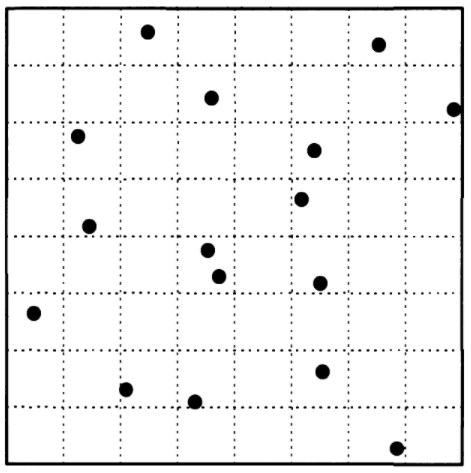
\includegraphics[scale=0.4]{Malla.png}
    \caption{Esquema de la división de la taza de café con moleculas distribuidas aleatoriamente después de determinado tiempo.}
    \label{Esquema}
\end{figure}

\section*{Marco teórico}

El presente proyecto se fundamenta en la entropía y la segunda ley de la termodinámica, que se basa en el hecho de que existen muchos más estados desordenados que ordenados. De forma que, si un sistema comienza de forma ordenada, con el paso del tiempo evolucionará y su estado cambiará de acuerdo a las leyes de la física. Si se sigue recorriendo la flecha del tiempo existe una probabilidad alta de que el estado esté más desordenado. Por lo que, si el sistema cumple la condición de orden elevado tenderá a aumentar su desorden con el tiempo y a esto se le llamará la entropía. De forma estadistica se define como:

\begin{equation}
        \sum_{i=1}=P_i ln(P_i)
        \label{Entropía}
\end{equation}

Donde Pi es la probabilidad de encontrar el sistema en estado i. Después de un tiempo el sistema se aproxima al equilibrio. Esto ocurre debido a que el sistema explora todos los estados disponibles con la misma probabilidad. Lo anterior debido a la hipótesis de Ergodic, la cual juega un importante rol en física estadística. 




\section*{Análisis y resultados}

\subsection*{Primer punto: Entropía del sistema y gráfica de resultados} 

Se calculó la entropía para una malla de tamaño 20, es decir 400 cuadrículas y con 100000 pasos.

\begin{figure}[H]
    \centering
    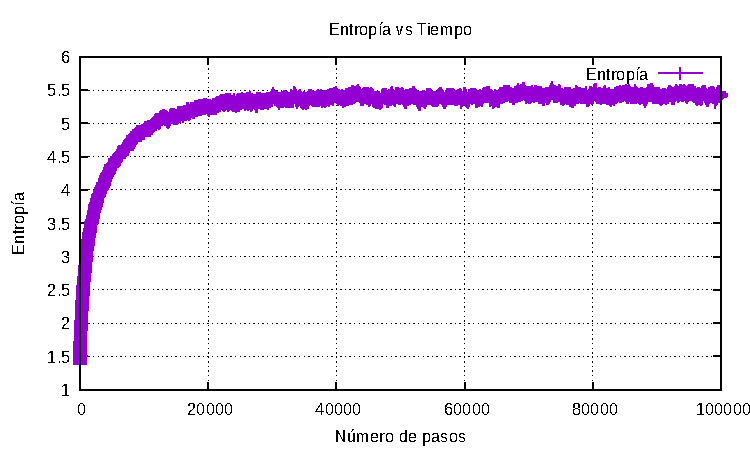
\includegraphics[width=\columnwidth]{punto_1.pdf}
    \caption{Entropía del sistema}
    \label{Entropia}
\end{figure}

Como podemos visualizar en la figura \ref{Entropia}, la entropía va aumentando con el tiempo, ya que se le están agregando pasos y al final tiende a un estado de equilibrio.



\subsection*{Segundo punto: Entropía en función del tiempo con diferentes tamaños}

Cambiando los tamaños de la malla se calculó la entropía experimental y teórica. En la figura \ref{Entropia_varios_tamaños}  podemos ver un comportamiento creciente parecido al cuadrático, como es esperado.

\begin{figure}[H]
    \centering
    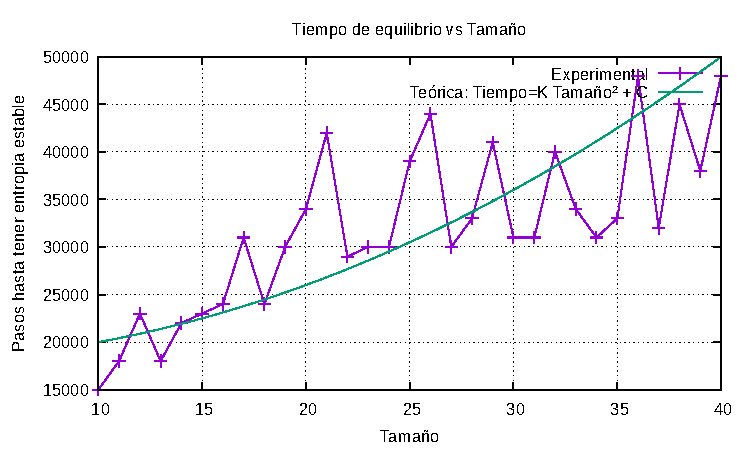
\includegraphics[width=\columnwidth]{punto_2.pdf}
    \caption{Entropía del sistema para diferentes tamaños, tanto experimental como teórica}
    \label{Entropia_varios_tamaños}
\end{figure}

\subsection*{Tercer punto: Simulación de una caminata aleatoria de las párticulas midiendo tamaño de la gota}

En este caso, se usó la fórmula

\begin{equation}
    \Omega = \sqrt{\frac{\sum r_i^2}{N}}
\end{equation}

Donde $\Omega$ es el tamaño de la gota de crema. 

Como parámetros se usaron: Una taza de 100 x 100 unidades, 100 particulas y 10000 pasos



\begin{figure}[H]
    \centering
    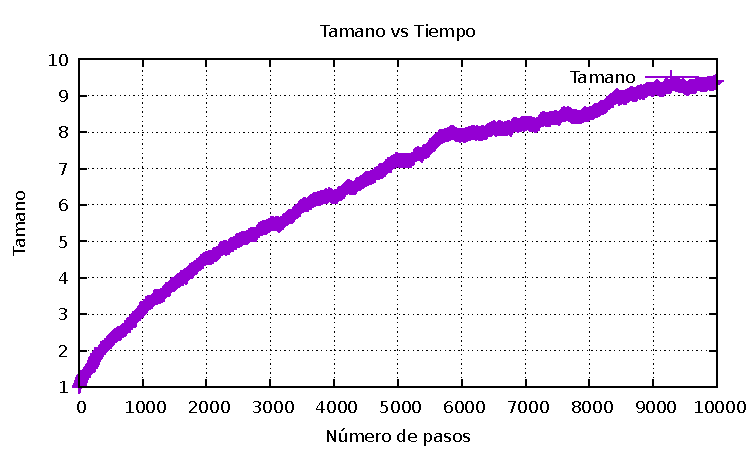
\includegraphics[width=\columnwidth]{punto_3.pdf}
    \caption{Tamaño de la gota}
    \label{tamaño_gota}
\end{figure}

Como se puede visualizar, el comportamiento es proporcional a $\sqrt{t}$. En la simulación hecha, la constante de proporcionalidad es de aproximadamente $1/10$.

\subsection*{Cuarto punto: Simulación con agujeros en las paredes}

Para la simulación de la taza con hueco se usaron los siguientes parametros: Una caja de 50x50 unidades, 400 partículas y 200000 pasos. Se obtuvo la figura  \ref{numero_particulas}.



\begin{figure}[H]
    \centering
    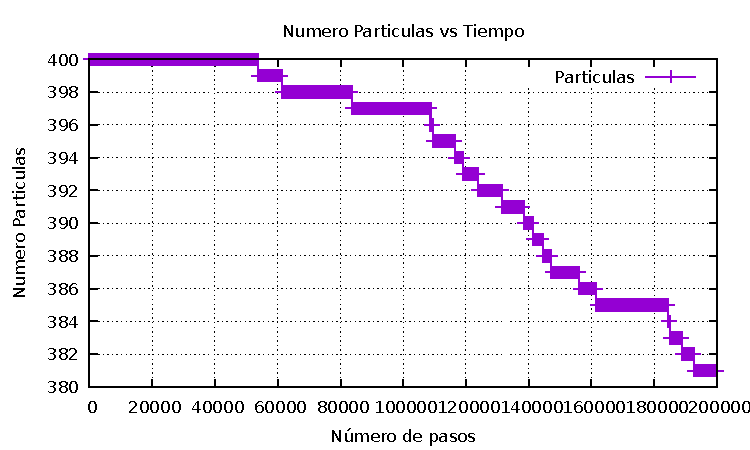
\includegraphics[width=\columnwidth]{punto_4.pdf}
    \caption{Número de partículas}
    \label{numero_particulas}
\end{figure}

Como podemos ver el número de particulas va decreciendo con el tiempo, precisamente por lo que las paredes son huecos, por lo que la gŕafica describe correctamente el sistema.

\subsection*{Optimización}

Se realiza la figura \ref{optimizacion}, en la que se visualiza el tiempo empleado en el código para diferentes tamaños, desde 10 hasta 100, para así comparar el impacto de la optimización, en este caso -O3.
 
 \begin{figure}[H]
    \centering
    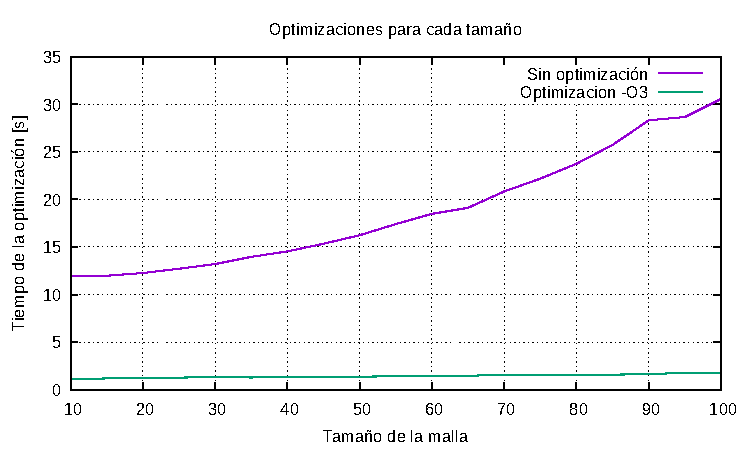
\includegraphics[width=\columnwidth]{optimizacion.pdf}
    \caption{Tiempo empleado en el código para diferentes tamañoz con y sin optimización}
    \label{optimizacion}
\end{figure}

Como podemos ver hay una diferencia amplia entre usar el código con o sin implementación, viendo que la mejora es de casi el $95\%$.
 
\section*{Dificultades y soluciones}

1. Se presentaron varios códigos como propuesta para la solución de los problemas, Al final, se escogió la mejor y más conveniente. 

2. Como la mayoría de puntos manejan un alto cambio de parámetros, decidimos manejarlos de forma independiente en cada código. Por lo cual se decidió usar los parámetros del archivo input.txt únicamente para el primer punto, en el que tenía más sentido y mayor facilidad.

3. Se presentó dificultades en cómo recorrer la matriz de casillas para conocer la entropía, ya que existen dos formas de hacerlo, por preferencia de filas o columnas. Se analizó el tiempo con Perf, encontrando un resultado similar para ambos casos, por lo que se siguió indagando y se encontró que la mejor forma de hacerlo era con el índice $i$ del propio de Eigen. Con esto se logró que el tiempo de ejecución redujera aproximadamente al $50\%$ gracias al uso de (Matriz.data()+i).

4. Otra cosa que pudimos visualizar al momento de ejecución es que, gracias a el informe de Gprof, el mayor tiempo de ejecución es usado en la creación de números aleatorios. Para solucionar esto se propuso la optimización en la función Step. Después se intentó con la función Step\_2, sin embargo, no se redujo considerablemente el tiempo, se ayudó en 1 parte entre 40 del tiempo anterior.

5. En el punto 2 se presentó dificultades para la obtención de la gráfica, ya que es distante de los datos teóricos. La entropía, a pesar de ser estable, no se describe estática en la simulación, los valores tienen una gran incertidumbre que se va propagando y por eso se ven afectados los datos.

\section*{Conclusiones}

1. La entropía va creciendo con el paso del tiempo y al final tiende a un estado de equilibrio.

2. A medida que se recorre la flecha del tiempo para diferentes tamaños, la entropía se comporta de forma creciente.

3. El tamaño de la gota de crema crece de forma proporcional a $\sqrt{t}$.

4. Si la malla adquiere un comportamiento de huecos en las orillas, el sistema tiende a decrecer en el número de partículas.

5. Es claro que el tiempo del comportamiento descrito mejora usando optimizaciones.

\end{multicols}


\end{document}
